\section{Proof of Eq.~\eqref{equ.Pick_sim-con}}\label{appendix:Pick}
\begin{figure}
    \centering
    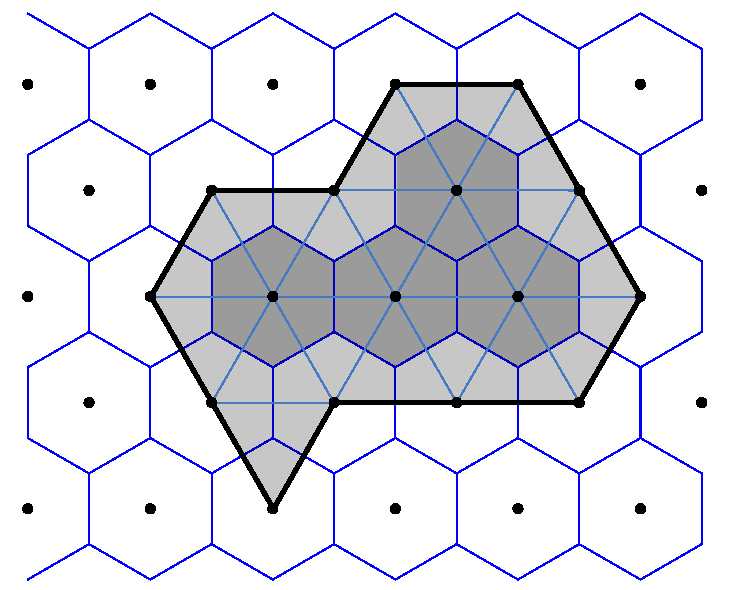
\includegraphics[width=0.6\linewidth]{figures/dual-lattice-Pick-theorem.pdf}
    \caption{A triangular lattice and a honeycomb lattice are dual to each other, in the sense that each lattice point of a system is at the center of a face of the other one. The boundary $C=\de A$ of the shaded region $A$ is a \textit{circuit} defined in the triangle lattice. As shown above, $A$ consists of $f$ faces of the triangular lattice, where each face corresponds to a vertex of the dual honeycomb lattice, indicating $f=N^A$. The darker region consists of $N^A_p$ hexagons entirely inside $A$, which is equivalent to counting the number of vertices $v$ of the triangular lattice enclosed by $C$. The length $\ell\equiv\abs{C}$ of the circuit can be understood as the number of edges in the honeycomb lattice that cross $C$. }
    \label{fig.dual-lattice-Pick-theorem}
\end{figure}
We find it more convenient to prove the formula by mapping the original honeycomb lattice to its dual triangular lattice, because a theorem on this problem has been discussed for triangular lattices~\cite{Lieb-Loss_1992}. 

A \textit{circuit} $C$ of length $\ell$ in a lattice is defined as an ordered sequence of distinct sites $i_1,\cdots, i_\ell$ with the periodic property that $(i_n, i_{n+1})$ is an edge for $n = 1, \cdots, \ell$ with $i_{\ell+1} \equiv i_1$, and the area enclosed by $C$ is denoted by $A$, which is simply-connected. Consider a triangular lattice. Lemma 2.3 of~\cite{Lieb-Loss_1992} gives the following equation
\begin{equation}\label{equ.Lieb-Loss-formula}
    \ell = f - 2v + 2
\end{equation}
where $f$ and $v$ denote the number of interior \textit{faces} and \textit{vertices} of $A$, respectively, and $\ell\equiv\abs{C}$ is the length of the circuit. See \autoref{fig.dual-lattice-Pick-theorem} for an illustration. In the figure, it is also clearly shown that the dual lattice of a triangular lattice is a honeycomb lattice, which is the geometry of our interest in this work. The duality gives several correspondences between the triangular and honeycomb lattices, which are $\ell\leftrightarrow\abs{\de A}$, $f\leftrightarrow N^A$, and $v\leftrightarrow N^A_p$. Replacing quantities in \eqref{equ.Lieb-Loss-formula} defined in a triangular lattice by their corresponding quantities defined in the dual honeycomb lattice, e.g. $\abs{\de A}$, $N^A$, and $N^A_p$, according to these correspondences, gives
\[
\abs{\de A} = N^A - 2N^A_p + 2
\]
This proves Eq.~\eqref{equ.Pick_sim-con}.

This formula can be generalized to multiply-connected regions. Suppose a connected region has a genus number $g$, and the $n$-th hole surrounded by the connected region $A$ is denoted by $B^{(n)}$ such that $A\cap B^{(n)}=\varnothing$ and $A\cup \lr{\bigcup_{n=1}^{g} B^{(n)}}$ is simply-connected. Denoting by $\ell_{\mrm{out}} = \abs{\de\lr{A\cup \lr{\bigcup_{n=1}^{g} B^{(n)}}}}$ the number of crossing edges of the outer boundary, and by $\ell_{\mrm{in}}^{(n)}=\abs{\de B^{(n)}}$ the length of the $n$-th inner boundary, we have
\[
\left\{
\begin{aligned}
&\ell_{\mrm{out}} = N^A- 2N^A_{p} + \sum_{n=1}^{g}\lr{N^{B(n)} -2N^{B(n)}_{p} - 2N^{\de(n)}_{p}} +2 \\
&\ell_{\mrm{in}}^{(n)} = N^{B(n)} -2N^{B(n)}_{p}  +2
\end{aligned}
\right.
\]
where $N^{\de(n)}_p$ is the number of plaquettes at the interface between $A$ and $B$. It is obvious that $N^{\de(n)}_p = \ell_{\mrm{in}}^{(n)}$. Thus, we have
\[
\ell_{\mrm{out}} = N^A- 2N^A_{p} - \sum_{n=1}^{g}\ell_{\mrm{in}}^{(n)} -2g + 2
\]
At the same time, we know that the length of the boundary of the region $A$ is the sum of the outer boundary and all inner boundaries
\[
\abs{\de A} = \ell_{\mrm{out}} + \sum_{n=1}^{g}\ell_{\mrm{in}}^{(n)}
\]
Combining this relation with the result we obtained gives a generalized version of Eq.~\eqref{equ.Pick_sim-con}:
\[
\abs{\de A} = N^A-2N^A_p+2(1-g)
\]
